% !TEX root = ../main.tex

\section{How it works?}

\begin{figure}[H]
  \centering
  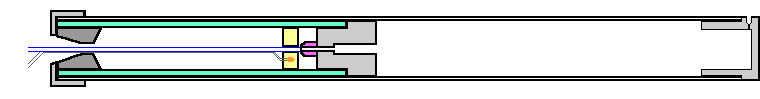
\includegraphics[width=0.8\textwidth,height=2.5cm,keepaspectratio]{seq01.png}
  \caption{Empty motor}
  \label{fig:emptyMotor}
\end{figure}

\begin{figure}[H]
  \centering
  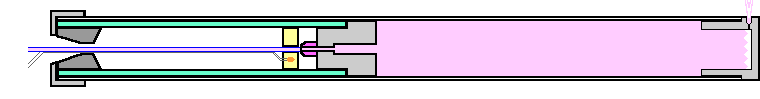
\includegraphics[width=0.8\textwidth,height=2.5cm,keepaspectratio]{seq04.png}
  \caption{Motor filled with $N_2O$ and venting}
  \label{fig:filledMotor}
\end{figure}

\begin{figure}[H]
  \centering
  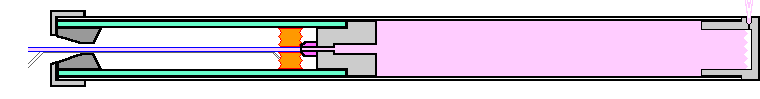
\includegraphics[width=0.8\textwidth,height=2.5cm,keepaspectratio]{seq06.png}
  \caption{The ignitor starts the combustion of the solid grain}
  \label{fig:startSolidBurnMotor}
\end{figure}

\begin{figure}[H]
  \centering
  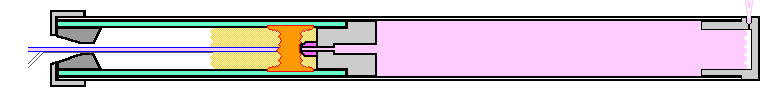
\includegraphics[width=0.8\textwidth,height=2.5cm,keepaspectratio]{seq08.png}
  \caption{The combustion of the solid grain burns the gas tube}
  \label{fig:solidBurningMotor}
\end{figure}

\begin{figure}[H]
  \centering
  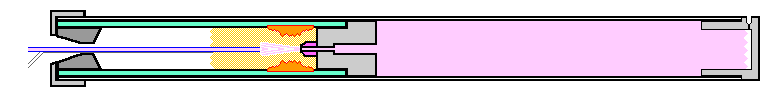
\includegraphics[width=0.8\textwidth,height=2.5cm,keepaspectratio]{seq09.png}
  \caption{The gas leaks through the tube}
  \label{fig:gasLeakingMotor}
\end{figure}

\begin{figure}[H]
  \centering
  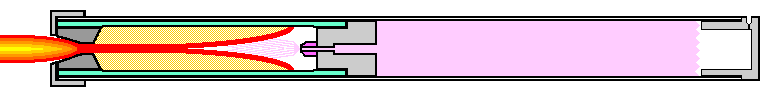
\includegraphics[width=0.8\textwidth,height=2.5cm,keepaspectratio]{seq10.png}
  \caption{The motor is now functioning}
  \label{fig:functioningMotor}
\end{figure}
